% Drawing 31/04-1 -- folder 31, batch 04, archive page 67 (PDF page 68).
% Transcription: à gauche, au bas de la page, un croquis du plan $(p,q)$ : les deux axes ; une droite oblique descendant du haut de l'axe des $q$ vers l'axe des $p$, avec des croix le long d'elle et sur l'axe des $q$ ; des croix le long de l'axe des $p$, qui se prolonge en tirets ; sous l'axe, « $\varphi(x)$ » et « $\varphi(x)+1$ », précédés d'une étiquette surchargée
% Kind: sketch of the (p,q) plane of a spectral sequence. Method 2 (schematic redraw from the facsimile). Status: partial.
% Notes: Ink. Axes; the oblique line from the top of the q-axis, which stops just above the p-axis; crosses on the q-axis (one heavy at the top), four along the oblique line, and along the p-axis, the last three on the dashed continuation; phi(x) and phi(x)+1 under the first two of these. Still differs: a first label under the foot of the oblique line is overwritten (it looks like phi(x) = phi(x) - 1 or phi(x) - 1) and is left out. The transcription's note places the sketch in the right margin; it is at the lower left of the page. Redrawn 2026-11-12 (issue 128): to check again.
% Coordinates: 1 unit = 1 mm = 1/100 of the crop width (bbox in page fractions: [0.14, 0.63, 0.52, 0.8]).
% Redrawn by Claude (claude-fable-5-2), issue #128, 2026-11-12; not checked by a human; not compiled (no TeX in the session).
% Rights: reproduces part of the work -- behind RENDER_TRANSCRIPTS, never published by itself.
\documentclass[tikz,border=3pt]{standalone}
\usepackage{amsmath,amssymb}
\usetikzlibrary{patterns,arrows.meta}
\tikzset{pencil/.style={black!45}, struck/.style={black!35}, mpt/.style={circle,draw,inner sep=1.3pt}, pt/.style={circle,fill,inner sep=0.9pt}, opt/.style={circle,draw,fill=white,inner sep=1.1pt}}
\begin{document}
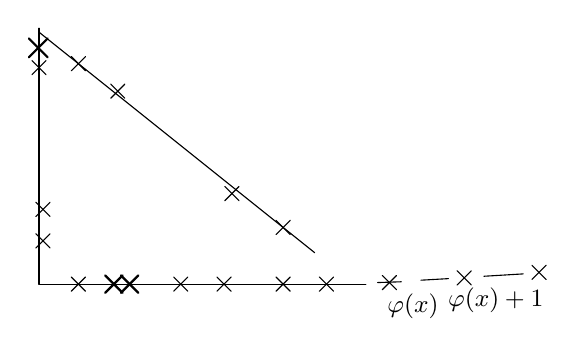
\begin{tikzpicture}[x=1mm,y=1mm,line cap=round,line join=round,font=\scriptsize]
\draw (19.5,-16) -- (19.5,-48.5) -- (61,-48.5);
\draw (62.5,-48.3) -- (65.5,-48.2);
\draw (68,-48) -- (71.5,-47.8);
\draw (76,-47.5) -- (81,-47.2);
\draw (19.5,-16.5) -- (54.5,-44.5);
\draw[thick] (18.2,-17.3) -- (20.6,-19.7);
\draw[thick] (18.2,-19.7) -- (20.6,-17.3);
\draw (18.6,-20.1) -- (20.4,-21.9);
\draw (18.6,-21.9) -- (20.4,-20.1);
\draw (19.1,-38.1) -- (20.9,-39.9);
\draw (19.1,-39.9) -- (20.9,-38.1);
\draw (19.1,-42.1) -- (20.9,-43.9);
\draw (19.1,-43.9) -- (20.9,-42.1);
\draw (23.6,-19.6) -- (25.4,-21.4);
\draw (23.6,-21.4) -- (25.4,-19.6);
\draw (28.6,-23.1) -- (30.4,-24.9);
\draw (28.6,-24.9) -- (30.4,-23.1);
\draw (43.1,-36.1) -- (44.9,-37.9);
\draw (43.1,-37.9) -- (44.9,-36.1);
\draw (49.6,-40.4) -- (51.4,-42.2);
\draw (49.6,-42.2) -- (51.4,-40.4);
\draw (23.6,-47.6) -- (25.4,-49.4);
\draw (23.6,-49.4) -- (25.4,-47.6);
\draw (36.6,-47.6) -- (38.4,-49.4);
\draw (36.6,-49.4) -- (38.4,-47.6);
\draw (42.1,-47.6) -- (43.9,-49.4);
\draw (42.1,-49.4) -- (43.9,-47.6);
\draw (49.6,-47.6) -- (51.4,-49.4);
\draw (49.6,-49.4) -- (51.4,-47.6);
\draw (55.1,-47.6) -- (56.9,-49.4);
\draw (55.1,-49.4) -- (56.9,-47.6);
\draw (63.1,-47.4) -- (64.9,-49.2);
\draw (63.1,-49.2) -- (64.9,-47.4);
\draw (72.6,-46.8) -- (74.4,-48.6);
\draw (72.6,-48.6) -- (74.4,-46.8);
\draw (82.1,-46.1) -- (83.9,-47.9);
\draw (82.1,-47.9) -- (83.9,-46.1);
\draw[thick] (27.9,-47.4) -- (30.1,-49.6);
\draw[thick] (27.9,-49.6) -- (30.1,-47.4);
\draw[thick] (29.9,-47.4) -- (32.1,-49.6);
\draw[thick] (29.9,-49.6) -- (32.1,-47.4);
\node[inner sep=1pt] at (67,-51.3) {\small $\varphi(x)$};
\node[inner sep=1pt] at (77.5,-50.6) {\small $\varphi(x)+1$};
\end{tikzpicture}
\end{document}
